  \begin{frame}{Karte - Idee}
    \begin{itemize}
        \item Einfacher Weg die Stadt kennenzulernen
        \item Gut mit Vorwissen verbindbar
        \item geographisch relevante Daten
    \end{itemize}
  \end{frame}
  \begin{frame}{Karte - Prototyp}
    \begin{center}
        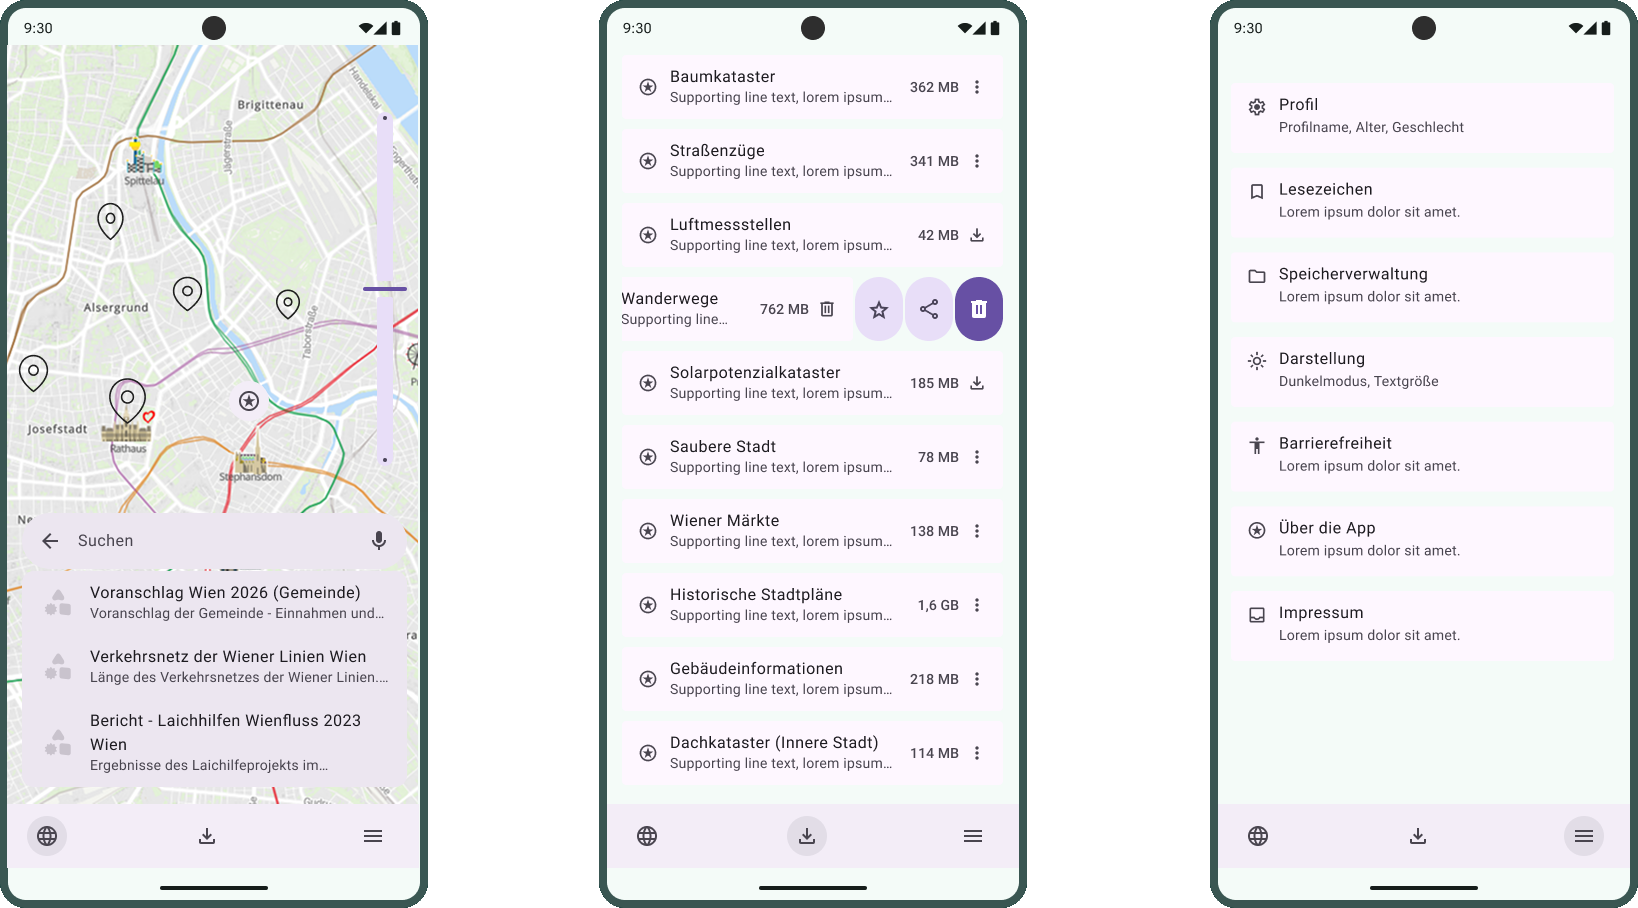
\includegraphics[width=\textwidth]{images/prototype_leonidas.png}
    \end{center}
  \end{frame}
  \begin{frame}{Karte - Anpassung}
    \begin{itemize}
        \item{Benjamin:} Verbesserte Suche
        \item{Leah:} Größe der Pins von Popularität abhängig
    \end{itemize}
  \end{frame}
  \begin{frame}{Evaluierung - Bruder}
  \end{frame}
  \begin{frame}{Evaluierung - KI-Feedback}
    \textbf{St\"{a}rken}
    \begin{itemize}
       \item Gut mit dem Alltag verbindbar
       \item Schönes Design
    \end{itemize}
    \textbf{Schw\"{a}chen}
    \begin{itemize}
        \item Kann unübersichtlich werden
        \item Teils schlechte Namensgebung
    \end{itemize}
  \end{frame}